\documentclass[border=6pt]{standalone}
\usepackage{tikz}
\usepackage[edges]{forest}
\usetikzlibrary{arrows.meta,positioning,calc,decorations.pathreplacing,shapes.geometric}
\begin{document}
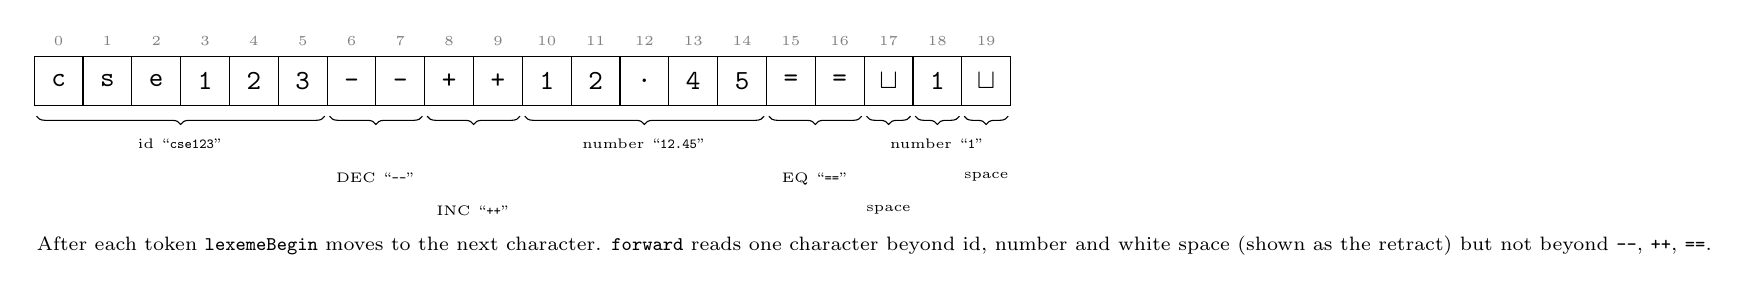
\begin{tikzpicture}[font=\small,cell/.style={draw,minimum size=0.62cm,inner sep=0pt,font=\ttfamily}]
\node[cell] at (0.00,0) {c};
\node[font=\tiny,gray] at (0.00,0.5) {0};
\node[cell] at (0.62,0) {s};
\node[font=\tiny,gray] at (0.62,0.5) {1};
\node[cell] at (1.24,0) {e};
\node[font=\tiny,gray] at (1.24,0.5) {2};
\node[cell] at (1.86,0) {1};
\node[font=\tiny,gray] at (1.86,0.5) {3};
\node[cell] at (2.48,0) {2};
\node[font=\tiny,gray] at (2.48,0.5) {4};
\node[cell] at (3.10,0) {3};
\node[font=\tiny,gray] at (3.10,0.5) {5};
\node[cell] at (3.72,0) {\char`\-};
\node[font=\tiny,gray] at (3.72,0.5) {6};
\node[cell] at (4.34,0) {\char`\-};
\node[font=\tiny,gray] at (4.34,0.5) {7};
\node[cell] at (4.96,0) {+};
\node[font=\tiny,gray] at (4.96,0.5) {8};
\node[cell] at (5.58,0) {+};
\node[font=\tiny,gray] at (5.58,0.5) {9};
\node[cell] at (6.20,0) {1};
\node[font=\tiny,gray] at (6.20,0.5) {10};
\node[cell] at (6.82,0) {2};
\node[font=\tiny,gray] at (6.82,0.5) {11};
\node[cell] at (7.44,0) {.};
\node[font=\tiny,gray] at (7.44,0.5) {12};
\node[cell] at (8.06,0) {4};
\node[font=\tiny,gray] at (8.06,0.5) {13};
\node[cell] at (8.68,0) {5};
\node[font=\tiny,gray] at (8.68,0.5) {14};
\node[cell] at (9.30,0) {=};
\node[font=\tiny,gray] at (9.30,0.5) {15};
\node[cell] at (9.92,0) {=};
\node[font=\tiny,gray] at (9.92,0.5) {16};
\node[cell] at (10.54,0) {$\sqcup$};
\node[font=\tiny,gray] at (10.54,0.5) {17};
\node[cell] at (11.16,0) {1};
\node[font=\tiny,gray] at (11.16,0.5) {18};
\node[cell] at (11.78,0) {$\sqcup$};
\node[font=\tiny,gray] at (11.78,0.5) {19};
\draw[decorate,decoration={brace,amplitude=3pt,mirror}] (-0.28,-0.45) -- (3.38,-0.45);
\draw[decorate,decoration={brace,amplitude=3pt,mirror}] (3.44,-0.45) -- (4.62,-0.45);
\draw[decorate,decoration={brace,amplitude=3pt,mirror}] (4.68,-0.45) -- (5.86,-0.45);
\draw[decorate,decoration={brace,amplitude=3pt,mirror}] (5.92,-0.45) -- (8.96,-0.45);
\draw[decorate,decoration={brace,amplitude=3pt,mirror}] (9.02,-0.45) -- (10.20,-0.45);
\draw[decorate,decoration={brace,amplitude=3pt,mirror}] (10.26,-0.45) -- (10.82,-0.45);
\draw[decorate,decoration={brace,amplitude=3pt,mirror}] (10.88,-0.45) -- (11.44,-0.45);
\draw[decorate,decoration={brace,amplitude=3pt,mirror}] (11.50,-0.45) -- (12.06,-0.45);
\node[font=\tiny,align=center,anchor=north,fill=white] at (1.55,-0.62) {id ``\texttt{cse123}''};
\node[font=\tiny,align=center,anchor=north,fill=white] at (4.03,-1.04) {DEC ``\texttt{{-}{-}}''};
\node[font=\tiny,align=center,anchor=north,fill=white] at (5.27,-1.46) {INC ``\texttt{++}''};
\node[font=\tiny,align=center,anchor=north,fill=white] at (7.44,-0.62) {number ``\texttt{12.45}''};
\node[font=\tiny,align=center,anchor=north,fill=white] at (9.61,-1.04) {EQ ``\texttt{==}''};
\node[font=\tiny,align=center,anchor=north,fill=white] at (10.54,-1.46) {space};
\node[font=\tiny,align=center,anchor=north,fill=white] at (11.16,-0.62) {number ``\texttt{1}''};
\node[font=\tiny,align=center,anchor=north,fill=white] at (11.78,-1.04) {space};
\node[font=\scriptsize,anchor=west] at (-0.4,-2.1) {After each token \texttt{lexemeBegin} moves to the next character. \texttt{forward} reads one character beyond id, number and white space (shown as the retract) but not beyond \texttt{--}, \texttt{++}, \texttt{==}.};
\end{tikzpicture}
\end{document}
